\documentclass{article}
\usepackage[dvipsnames]{xcolor}
\usepackage[paperwidth=20cm, paperheight=3.0cm, margin = 0cm, top=0.5cm]{geometry}

\usepackage{pgf}
\usepackage{tikz}
\usetikzlibrary{arrows,automata}
\usetikzlibrary{positioning}
\tikzstyle{source}  = 
[
	draw,circle,fill=black,thick,inner sep=0mm,minimum size=2mm
]

\tikzstyle{box}  =
[
	draw,rectangle,thick,inner sep=2mm,
	minimum width=8mm, minimum height=8mm
]

\tikzstyle{redbox} = 
[
	draw,rectangle,thick,inner sep=2mm,
	minimum width=8mm, minimum height=8mm,
	fill=red, opacity=0.3, text opacity=1, draw opacity=1
]

\tikzstyle{bluebox} = 
[
	draw,rectangle,thick,inner sep=2mm,
	minimum width=8mm, minimum height=8mm,
	fill=blue, opacity=0.3, text opacity=1, draw opacity=1
]

\tikzstyle{lgreenbox} = 
[
	draw,rectangle,thick,inner sep=2mm,
	minimum width=8mm, minimum height=8mm,
	fill=SpringGreen
]

\tikzstyle{bluestate}  = 
[
	state, draw=blue, line width=2pt,
	fill=LimeGreen
]

\tikzstyle{redstate}  = 
[
	state, draw=red, line width=2pt,
	fill=LimeGreen
]

\tikzstyle{violetstate}  = 
[
	state, draw=Violet, line width=2pt,
	fill=LimeGreen
]
 



\begin{document}
\begin{center}
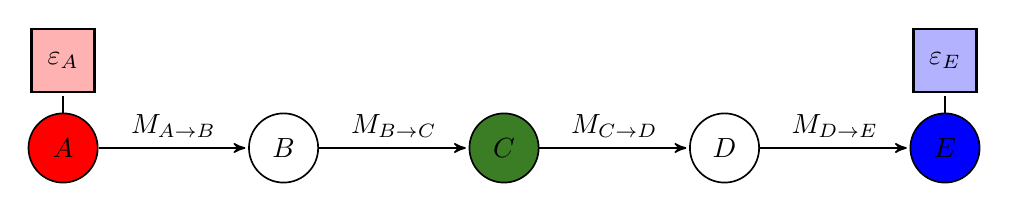
\begin{tikzpicture}[->,>=stealth',shorten >=1pt,auto,node distance=2.8cm,semithick]
                    
\node[state, fill=red] (X1)               {$A$}; 
\node[state] (X2) [right of=X1] {$B$};                   
\node[state, fill=OliveGreen] (X3) [right of=X2] {$C$};                   
\node[state] (X4) [right of=X3] {$D$};                   
\node[state, fill=blue] (X5) [right of=X4,] {$E$}; 

\node[redbox][above=0.25cm of X1](E1){$\varepsilon_A$};                  
\node[bluebox][above=0.25cm of X5](E5){$\varepsilon_E$};                  


\path
	(X1) edge node {$M_{A\to B}$} (X2)
	(X2) edge node {$M_{B\to C}$} (X3)
	(X3) edge node {$M_{C\to D}$} (X4)
	(X4) edge node {$M_{D\to E}$} (X5);

\path
	(X1) edge[-] (E1)
	(X5) edge[-] (E5);

\end{tikzpicture}
\end{center}

\end{document}
